\documentclass{article}
\usepackage{hyperref}
\usepackage{graphicx}
\usepackage{float} % here for H placement parameter

%All LaTeX documents have a ``preamble'' that includes the packages and macros needed to make the document compile. The file `PomonaLgcsFormatting.tex' includes the preamble for this template. You can see it in the file list on the left frame of your screen, and this document is instructed to use it with the \input{} command below.

% \input{PomonaLgcsFormatting}

\title{A Comparative Analysis of Distriuted File Systems}
\author{Projit Bandyopadhyay (20161014) \\ Siddharth Bhat (20161105) \\ Alok Debnath (20161122)}
\date{\today} 

\begin{document}

\maketitle

\begin{abstract}

Distributed file systems (DFSs) aim to provide an efficient and reliable storage solutions which are easily accessible, manageable and robust against data loss in case of failure, i.e. fault tolerant. Distributed file systems may also provide varying degrees of access of the servers and clients.In this project report, we extensively analyze and compare three different commonly known distributed file systems, the \textit{Google File System} (GFS), the \textit{Hadoop Distributed File System} (HDFS) and MinIO. We first introduce, analyze and describe some common properties of distributed file systems. We then introduce each of the aforementioned DFSs and finally, provide an in-depth comparison of these DFSs based on the metrics described. 

\end{abstract}

\section{Introduction}
\label{sec: intro}

A distributed file system (DFS) is a file system implemented on a client/server architecture, where one or more central servers store files that can be accessed by multiple remote clients, which is based on the access protocol defined by server and the level of access granted to the client. The fundamental feature of a distributed file system is that the interface of the file access by the remote client is as if the file is being accessed from their local machine. Therefore, files can be cached, accessed and managed on the local client machine, but the process is managed by a single, or a network of centralized servers.

DFSs constitute the primary support for data management. They provide an interface whereby to store information in the form of files and later access them for read and write operations. Among the several implementations of file systems, few of them specifically address the management of huge quantities of data on a large number of nodes. Mostly these file systems constitute the data storage support for large computing clusters, supercomputers, massively parallel architectures, and lately, storage/computing clouds \cite{buyya2013mastering}.

Distributed file systems allow for an efficient, easily manageable and extensible data storage and sharing given a network and relevant network protocols. As mentioned before, one of the key features of a DFS is the ability of the server to set up a protocol to restrict client access based. This allows multiple clients to be able to access multiple files hosted on a server with varying degrees of access. DFSs depend on three main notions of \textit{transparency, fault tolerance} and \textit{scalability}.

Transparency \cite{floyd1989transparency} implies the user should be able to access the distributed file system regardless of their login node or client machine, and based on their access level, should be able to perform the same operations, without caring about the faults in the system, because of the fault tolerant mechanisms of the distributed system itself. Therefore, the client should be able to access the requisite files without worrying about consistency, faults and the complexity of the underlying file system.

Fault tolerance \cite{becker1994application} should not be stopped in case of transient or partial failures. Faults could be of network failure or server failure, which would result in data and service unavailability, compromising data integrity. Fault tolerance plays an integral role in consistency when several users concurrently access the data, typically when the data is stored in multiple server locations. The cost and complexity of designing such systems increases significantly based on the severity of the failures and the relative importance of the data to to the server host(s).

Scalability \cite{mccreadie2012mapreduce} is the ability of efficiently leverage large amounts of servers, which can be either dynamically and continuously added to the system. A distributed file system should be scalable to account for maintaining replicas and increasing fault tolerance as the number of files, size of files or number of clients increase. Scalability implies both storage space as well as distributed compute. Some systems which adopt a centralized architecture provide tools such as multi-threading for scaling client access to files in DFSs.

\subsection{Terms and Jargon used in Distributed File System Literature}

The literature on DFSs is based on a combination of literature in distributed systems as well as local file system and computer system architecture. Therefore, a high density of jargon has evolved that is specific to this field. A few of these terms have been detailed here.


\subsubsection{High Availability}
High availability is that characteristic of a system, which aims to ensure an agreed level of operational performance, usually uptime, for a higher than normal period. This implies that a highly available system will:
    \begin{itemize}
        \item \textbf{Add redundancy} to remove single points of failure. One component failing shouldn't bring the system down.
        \item \textbf{Reliably crossover}. Given that the system is redundant, the crossover point is prevented, from becoming a single point of failure.
        \item \textbf{Limit the chances of failure}. Given the above two principles, failures shouldn't occur. If and when they do, they should be detected as soon as possible, and regular maintenance must be done. 
    \end{itemize}

\subsubsection{Shards}
A database shard is a horizontal partition of data in a database or search engine. Each individual partition is referred to as a shard or database shard. Each shard is held on a separate database server instance, to spread load.

The advantages of having shards include:
    \begin{itemize}
        \item Total rows per table reduced
        \item Index size reduced, improving search performance
        \item Distribute database over more hardware.
        \item Some data is naturally distributed like this (ex. country specific data stored in shard of database which is physically present in that country for lower network latency)
    \end{itemize}

However, there are some disadvantages as well, which are:
    \begin{itemize}
        \item Increased complexity of SQL
        \item Sharding introduces complexity
        \item Single point of failure
        \item Failover servers more complex
        \item Backups more complex
        \item Operational complexity added
    \end{itemize}

\subsubsection{Volumes}
Volumes are a management entity that logically organize a cluster’s data. Since a container always belongs to exactly one volume, that container’s replicas all belong to the same volume as well. Volumes do not have a fixed size and they do not occupy disk space until MapR file system writes data to a container within the volume. A large volume may contain anywhere from 50-100 million containers. Typical use cases include volumes for specific users, projects, development, and production environments. For example, if an administrator needs to organize data for a special project, the administrator can create a specific volume for the project. The MapR file system organizes all containers that store the project data within the project volume. A cluster can have many volumes.

Mirror volumes are read-only copies of a source volume. Mirror volumes can be promoted to read-write volumes. The main use case for this feature is to support disaster-recovery scenarios in which a read-only mirror needs to be promoted to a read-write volume so that it can become the primary volume for data storage. In addition, read-write volumes that were mirrored to other volumes can be made into mirrors (to establish a mirroring relationship in the other direction). You can also convert read-write volumes back to read-only mirrors.

\subsubsection{Snapshots}
Snapshots enable you to roll back to a known good data set. A snapshot is a read-only image of a volume that provides point-in-time recovery. Snapshots only store changes to the data present in the volume, and as a result make extremely efficient use of the cluster’s disk resources. Snapshots preserve access to historical data, and protect the cluster from user and application errors. You can create a snapshot manually, or automate the process with a schedule. 

\subsubsection{MapReduce}
MapReduce is a software framework that allows applications to be written for processing a large amount of data. MapReduce runs applications in parallel on a cluster of low-end machines in a reliable and fault-tolerant manner. It comprises a number of map and reduce tasks. Each task works on a part of data. This distributes the load across the cluster. The function of Map tasks is to load, parse, transform and filter data. Each reduce task works on the sub-set of output from the map tasks. Reduce task applies grouping and aggregation to this intermediate data from the map tasks.

The input file for the MapReduce job exists on HDFS. The inputformat decides how to split the input file into input splits. Input split is nothing but a byte-oriented view of the chunk of the input file. This input split gets loaded by the map task. The map task runs on the node where the relevant data is present. The data need not move over the network and get processed locally.

\subsection{Types of Distributed File Systems}

By architecture design, DFSs can be classified as \textbf{Client-Server Architectures} and \textbf{Cluster-Based Distributed File System}. 
\begin{itemize}
    \item A client-server architectures have several servers which manage the data store and caching functions, access management and data transfer between different clients. The data transfer and the metadata are not decoupled, meaning that the data access is based on a global namespace, which is shared by multiple clients. In a client-server architecture, the addition of new servers increases processing capacity as well as storage.
    
    \item On the contrary, a cluster based distributed file system decouples the metadata and the data transfer, by having dedicated servers to manage storage and others to manage metadata. Increasing the number of storage servers increases the overall capacity of the distributed system, but might negatively effect the query time if the metadata server(s) are not increased in capacity. Systems having a single metadata server are referred to as centralized cluster based DFSs and often have a single point of failure. Distributed metadata servers occur in totally distributed cluster based DFSs
\end{itemize}

In terms of cache consistency, the distributed systems can be analyzed as systems that implement \textit{Write Once Read Many (WORM)}, \textit{Transactional Locking} and \textit{Leasing} \cite{reed1996analysis}. 

\begin{itemize}
    \item Write Only Read Many (WORM) is an approach that ensures mutual consistency across the servers and clients based on single write to a file segment which can then be accessed multiple times for reading.  Once a file is created, it cannot be modified, rewritten or appended.  Cached files are in read-only mode, therefore each read reflects the latest version of the data. Consistency here mirrors guaranteed eventual consistency in distributed systems as the final version of a file is going to be the same and therefore a file which is being written can not be read at the same time as it is being appended by a single client. Note that this is only for the version of the file which is cached at a single server.
    
    \item Transactional locking implies the obtaining of a read lock on the requested data, so that any other users cannot perform a write on this data; or obtaining a write lock in order to prevent any reads or writes on this data. Therefore, each read reflect the latest write, and each write is done in order. In transactional locking, the idea is to update all copies of a data in cache when one them is modified in order to improve the performance of the system, while locking the read such that it can only reflect the latest write.
    
    \item Leasing is another approach to cache consistency, where the server and client are locked in an intermittent contract. This lease is provided when the data is requested by the client and the lease grants exclusive access to a client on that file, Therefore, no other clients can request that file when it is being read or written by any client. This system can be modified to functioning on parts of a file rather than a single file, which would make a single file accessible in sections to multiple clients.
\end{itemize}

DFSs may also be categorized by how they synchronize between copies of the data. This must be accounted for when data is rewritten, and all of its copies must be updated to provide users with the latest version of the data. Currently, three main approaches exist for synchronization in distributed file systems in case of a partial or total rewrite, which are \textit{synchronous, asynchornous} and \textit{semi-asynchronous}

\begin{itemize}
    \item In the synchronous method, any request on modified data is blocked until all the copies are updated.  This ensures the users access the latest version of the data, but delays queries executions. This means that after the block of data is modified, each copy of that block updates at the same time, stalling queries which come when the synchronization is underway. From a distributed systems perspective, this system chooses to compromise availability for consistency.
    
    \item In the second method called asynchronous, requests on modified data are allowed, even if copies are not updated.  This way, requests could be performed in a reason-able time, but users can access to an out-of-date copy. However, this model allows access to the file whether or not a copy of it has been updated or not. Therefore, this system chooses to compromise consistency for availability, given a guarantee of eventual consistency.
    
    \item The last approach is a trade-off between the first two.  In the semi-asynchronous method,  requests are blocked until some copies, but not all, are updated. For example, let assume there are five copies of a data, a request on this data will be allowed once three copies will be updated.  This limits the possibility to access to an out-of-date data, while reducing delay for queries executions. Therefore, this method opts for availability if the client request is made after a copy has been updated and consistency in the case the copy has not been updated, therefore stalling only a fraction of the client requests.
\end{itemize}

\subsection{Metrics of Comparisons}

% \citep{depardon2013analysis}
is a seminal paper on the comparison of various popular file systems, where they analyzed the performance of six distributed file systems based on metrics essential to the scalablity, usability, consistency, security and deployability of distributed file systems. We use their metrics for analyzing distributed file systems in our report.

Each distributed file system is introduced on the basis of their naming, architecture, client and API access, cache consistency, replication, load balancing and fault detection. Naming is the mapping of the logical name of a file (and its path) to its physical location in memory. Given that is a DFS, server names holding the disk on which the data is stored need to be added, location transparency becomes key to the usability of a DFS. Fault detection, on the other hand, is the ability to detect overload servers, inconsistent behavior, corrupted data, and incorrect access for files by malicious clients, and plays an integral part in the scalability, usability and security of the DFS. Replication and load balancing are also important characteristics, as they are responsible for maintaining backups of the data in case of a crash and maintaining the balance of the server side on the addition and removal of servers in a transparent and consistent manner.

The metrics used in literature include:
\begin{itemize}
    \item \textit{scalability}, which looks into some analysis of the architecture to understand the ease with which a new server can be added to or removed from the DFS, and how the size of the files effects the nature of the architecture, such as, if a file exceeds the size possible to allocate to it on a storage server.
    
    \item \textit{transparency} analyses the DFS from the perspective of the client. Is the internal architecture abstracted from the client? Is there a transparency in file access, file operations and file caching? Is system transparency maintained in the case of a fault being detected? Finally, is the client access to the system performed in a transparent manner which is safe from a malicious clients?
    
    \item \textit{fault tolerance} studies the number of fail points of a DFS, and looks at the system consistency in case of a partial or complete overhaul. Is the data available in the event of a server failure? Is the data copy being accessed synchronized? Is the overall system well load balanced, in the case of the removal and/or addition of a server, and does it remain accessible during rebalancing the load in the presence of a new data server. Finally, is the caching protocol designed such that it is consistent with the latest copy of the file on the server?
\end{itemize}

In this report, we introduce and review some of the major components of three different DFSs with three different architectures, which are the Hadoop Distributed File System, the Google File System, and a rather novel DFS, MinIO.

\section{Hadoop Distributed File System (HDFS)}

The Hadoop Distributed File System \cite{borthakur2007hadoop} (HDFS) is a designed to be accessible and executable on commodity hardware. This implies that Hadoop is not only extensible and easily usable by consumer end machine networks, and can be hosted easily by low performance servers. It has multiple similarities with currently active distributed file systems, including the WORM model of computation discussed above, and the assumption of persistent failure modes. However, the differences from other distributed file systems are considerable in that HDFS is highly fault-tolerant and is designed to be deployed on low-cost hardware (hence a commodity distributed file system).

HDFS is a centralized distributed file system where the metadata is managed by a single server. This server provides a persistent copy of this metadata server information, which is interesting as it can allow on-the-fly restart with an up-to-date configuration and migration of the metadata informatin from the secondary to the primary data node.

HDFS provides high throughput access to application data and is suitable for applications that have large data sets. HDFS relaxes a few POSIX requirements to enable streaming access to file system data. HDFS was originally built as infrastructure for the Apache Nutch web search engine project. HDFS is part of the Apache Hadoop Core project.

Hadoop splits files into large blocks and distributes them across nodes in a cluster. It then transfers packaged code into nodes to process the data in parallel. This approach takes advantage of data locality, where nodes manipulate the data they have access to. This allows the dataset to be processed faster and more efficiently than it would be in a more conventional supercomputer architecture that relies on a parallel file system where computation and data are distributed via high-speed networking.

The Hadoop architecture is Open Source and is available at \url{http://hadoop.apache.org/}

\subsection{Goals of HDFS}

The aim of the Hadoop Distributed File System is to be implemented for hundreds of server nodes which are coupled with their data stores. Based on this, HDFS has the following goals:

\begin{itemize}
    \item \textbf{Speedy fault detection and reliability}: Hardware failure is the norm rather than the exception. An HDFS instance may consist of hundreds or thousands of server machines, each storing part of the file system’s data. The fact that there are a huge number of components and that each component has a non-trivial probability of failure means that some component of HDFS is always non-functional. Therefore, detection of faults and quick, automatic recovery from them is a core architectural goal of HDFS.
    
    \item \textbf{Streaming Data Access}: Applications that run on HDFS need streaming access to their data sets. HDFS is designed for batch processing rather than interactive use by users. Therwfore, there is a high empahsis on the throughput and data access rather rather than a low latency of data access. POSIX allows the imposition of multiple hard requirements that are not needed for applications that are targeted for HDFS. POSIX semantics in a few key areas has been traded to increase data throughput rates. 
    
    \item \textbf{Managing large datasets}: Applications which run on Hadoop typically have large data sets, in the order of giga to terabytes. Thus, HDFS is tuned to support large files. It should provide high aggregate data bandwidth and scale to hundreds of nodes in a single cluster. It should support tens of millions of files in a single instance.
    
    \item \textbf{Simple Coherency Model}: HDFS applications need a write-once-read-many (WORM) access model for files. A file once created, written, and closed should not need to be modified. This assumption simplifies data coherency issues and enables high throughput data access, as discussed above. A \textit{MapReduce} application or a web crawler application fits perfectly with this model.
    
    \item \textbf{Portability}: HDFS has been designed to be easily portable from one platform to another, for seamless cross-platform deployment. This facilitates widespread adoption of HDFS as a platform of choice for a large set of applications. 
\end{itemize}

\subsection{Architecture Description}

\begin{figure}
    \centering
    % \includegraphics[width=\linewidth]{HDFS.png}
    \caption{The Hadoop Distributed File System Architecture}
    \label{fig: hdfs}
\end{figure}

As seen in Figure \ref{fig: hdfs}, an HDFS cluster consists of a single \textbf{NameNode}, a master server that manages the file system namespace and regulates access to files by clients. Therefore, the NameNode is the master metadata and processing node. 

In addition, there are a number of \textbf{DataNodes}, usually one per node in the cluster. These DataNodes manage storage attached to the nodes that they run on. HDFS exposes a file system namespace which allows user data to be stored in files on each node. Internally, a file is split into multiple blocks, which are stored in a set of DataNodes. The NameNode executes file system namespace operations like opening, closing, and renaming files and directories. It also determines the mapping of blocks to DataNodes, and are therefore responsible for serving read and write requests from the file system’s clients. The DataNodes also perform block creation, deletion, and replication upon instruction from the NameNode. 

The NameNode and DataNode are designed to run on commodity and low-performance machines. These machines typically run a GNU/Linux operating system (OS). HDFS is built using Java; any machine that supports Java can run the NameNode or the DataNode software. Usage of the highly portable Java language means that HDFS can be deployed on a wide range of machines. A typical deployment has a dedicated machine that runs only the NameNode software. Each of the other machines in the cluster runs one instance of the DataNode software. The architecture does not preclude running multiple DataNodes on the same machine but in a real deployment that is rarely the case.

The existence of a single NameNode in a cluster greatly simplifies the architecture of the system. The NameNode is the arbitrator and repository for all HDFS metadata. The system is designed in such a way that user data never flows through the NameNode. A secondary NameNode is provided and is a persistent copy of the NameNode. This allows HDFS to restart with the latestconfiguration, in case of NameNode failures, by restoring the namespace from the secondary NameNode.

\subsubsection{Data Replication}

HDFS is designed to reliably store very large files across machines in a rather massive cluster. It stores each file as a sequence of blocks. The blocks of a file are to be replicated in order to improve the fault tolerance of the distrbuted file system. The block size and replication factor are configurable for each individual file, so they can be changed based on the importance associated with one file over another. All blocks in a file except the last block are the same size, while users can start a new block without filling out the last block to the configured block size after the support for variable length block was added to append and hsync. Therefore, the last block can be considered an overflow block.

An application can  choose to specify the number of replicas of a file. The replication factor can be specified at file creation time. It can be changed later, as files in HDFS are write-once (except for appends and truncates) and have strictly one writer at any time. Note that a truncate and an append are not considered file writes, as the file is segmented into blocks as mentioned before. Therefore, block rewrites are not allowed, which is where the efficiency of the WORM method is actually applicable. The NameNode makes all decisions regarding replication of blocks. It periodically receives a Heartbeat and a BlockReport from each of the DataNodes in the cluster. Receipt of a Heartbeat implies that the DataNode is functioning properly. A Blockreport contains a list of all blocks on a DataNode.

\paragraph{Replica Placement} The placement of replicas is critical to HDFS reliability and performance. Optimizing replica placement distinguishes HDFS as a unique DFS among its competitors, as it requires a lot of tuning and experience. The purpose of a rack-aware replica placement policy is to improve data reliability, availability, and network bandwidth utilization. The implementation for the replica placement policy, at the moment,  is a first effort in this direction.

Large HDFS instances run on a cluster of computers that commonly spread across many racks. Communication between two nodes in different racks has to go through multiple switches, which optmize on the distance between the NameNode and the DataNode. In most cases, network bandwidth between machines in the same rack is greater than network bandwidth between machines in different racks. The NameNode determines the rack id each DataNode belongs to via the process outlined in Hadoop Rack Awareness. A simple but non-optimal policy is to place replicas on unique racks, but while this prevents losing data when an entire rack fails and allows use of bandwidth from multiple racks when reading data, it is not vey efficient in the mapping of the rack bandwidths which could be clubbed together (and used to account for geographical closeness in ultra-wide networks). Therefore, a new policy evenly distributes replicas in the cluster which makes it easy to balance load on component failure is implemented. However, this policy increases the cost of writes because a write needs to transfer blocks to multiple racks.

Therefore, for the common case, when the replication factor is three, HDFS’s placement policy is to put one replica on the local machine if the writer is on a DataNode, otherwise on a random DataNode in the same rack as that of the writer, another replica on a node in a different (remote) rack, and the last on a different node in the same remote rack. This policy cuts the inter-rack write traffic which generally improves write performance. The chance of rack failure is far less than that of node failure; this policy does not impact data reliability and availability guarantees. 

\paragraph{Replica Selection} To optimize global bandwidth consumption and read latency, HDFS tries to satisfy a read request from a replica that is closest to the reader. Replicas on the same rack as the reader node are preferred. If HDFS cluster spans multiple data centers, then a replica which resides in the local data center is preferred.

\subsubsection{Metadata Persistence and Communication Protocols}

The HDFS namespace is stored by the NameNode. The NameNode uses a transaction log: \textit{the EditLog}; to persistently record the changes that occur in file system metadata. For example, creating a new file in HDFS causes the NameNode to insert a record into the EditLog. Similarly, a new record is inserted into the EditLog if the replication factor of a file is modified. The NameNode uses a file in its local host OS file system to store the EditLog. The entire file system namespace, including the mapping of blocks to files and file system properties, is stored in a file called the FsImage, which is stored as a file in the NameNode’s local file system.

The NameNode keeps an image of the entire file system namespace and file Blockmap in memory. When the NameNode starts up it reads the FsImage and EditLog from disk, applies all the transactions from the EditLog to the in-memory representation of the FsImage, and flushes out this new version into a new FsImage on disk. It can then truncate the old EditLog because its transactions have already been applied. This process is called ceckpointing. The purpose of a checkpoint is to make sure that HDFS has a consistent view of the file system metadata by taking a snapshot of the file system metadata and saving it to FsImage. Even though it is efficient to read a FsImage, it is not efficient to make incremental edits directly to a FsImage. Instead of modifying FsImage for each edit, we persist the edits in the EditLog.

The DataNode stores HDFS data in files in its local file system. The DataNode has no knowledge about HDFS files. It stores each block of HDFS data in a separate file in its local file system. The DataNode does not create all files in the same directory, rather it uses a heuristic to determine the optimal number of files per directory and creates subdirectories appropriately. When a DataNode starts up, it scans through its local file system, generates a list of all HDFS data blocks that correspond to each of these local files, and sends this report to the NameNode, known as the Blockreport.

All HDFS communication protocols are layered on top of the TCP/IP. A client establishes a connection to a configurable TCP port on the NameNode machine. It talks the ClientProtocol with the NameNode. The DataNodes talk to the NameNode using the DataNode Protocol. A Remote Procedure Call (RPC) abstraction wraps both the Client Protocol and the DataNode Protocol. By design, the NameNode never initiates any RPCs. Instead, it only responds to RPC requests issued by DataNodes or clients.

\subsection{Client Operations}

Data read request is served by HDFS, NameNode, and DataNode. Let's call the reader as a \texttt{client}. 

\subsubsection{Read Operations in HDFS}
\begin{enumerate}
    \item A client initiates read request by calling \verb|open()| method of \texttt{FileSystem} object; it is an object of type \texttt{DistributedFileSystem}.
    \item This object connects to NameNode using RPC and gets metadata information such as the locations of the blocks of the file. Note that these addresses are of first few blocks of a file.
    \item In response to this metadata request, addresses of the DataNodes having a copy of that block is returned back.
    \item Once addresses of DataNodes are received, an object of type \texttt{FSDataInputStream} is returned to the client. \texttt{FSDataInputStream} contains \texttt{DFSInputStream} which takes care of interactions with DataNode and NameNode. In step 4 shown in the above diagram, a client invokes \verb|read()| method which causes \texttt{DFSInputStream} to establish a connection with the first DataNode with the first block of a file.
    \item Data is read in the form of streams wherein client invokes \verb|read()| method repeatedly. This process of read() operation continues till it reaches the end of block.
    \item Once the end of a block is reached, \texttt{DFSInputStream} closes the connection and moves on to locate the next DataNode for the next block.
    \item Once a client has done with the reading, it calls a \verb|close()| method.
\end{enumerate}

\subsubsection{Write Operation In HDFS}
\begin{enumerate}
    \item A client initiates write operation by calling \verb|create()| method of DistributedFileSystem object which creates a new file.
    \item A \texttt{DistributedFileSystem} object connects to the NameNode using RPC call and initiates new file creation. However, this file creates operation does not associate any blocks with the file. It is the responsibility of NameNode to verify that the file (which is being created) does not exist already and a client has correct permissions to create a new file. If a file already exists or client does not have sufficient permission to create a new file, then \texttt{IOException} is thrown to the client. Otherwise, the operation succeeds and a new record for the file is created by the NameNode.
    \item Once a new record in NameNode is created, an object of type \texttt{FSDataOutputStream} is returned to the client. A client uses it to write data into the HDFS. Data write method is invoked (step 3 in the diagram).
    \item \texttt{FSDataOutputStream} contains \texttt{DFSOutputStream} object which looks after communication with DataNodes and NameNode. While the client continues writing data, \texttt{DFSOutputStream} continues creating packets with this data. These packets are enqueued into a queue which is called as \texttt{DataQueue}.
    \item There is one more component called \texttt{DataStreamer} which consumes this \texttt{DataQueue}. \texttt{DataStreamer} also asks NameNode for allocation of new blocks thereby picking desirable DataNodes to be used for replication.
    \item Now, the process of replication starts by creating a pipeline using DataNodes. In our case, we have chosen a replication level of 3 and hence there are 3 DataNodes in the pipeline.
    \item The \texttt{DataStreamer} pours packets into the first DataNode in the pipeline.
    \item Every DataNode in a pipeline stores packet received by it and forwards the same to the second DataNode in a pipeline.
    \item Another queue, \texttt{Ack Queue} is maintained by \texttt{DFSOutputStream} to store packets which are waiting for acknowledgment from DataNodes.
    \item Once acknowledgment for a packet in the queue is received from all DataNodes in the pipeline, it is removed from the \texttt{Ack Queue}. In the event of any DataNode failure, packets from this queue are used to reinitiate the operation.
    \item After a client is done with the writing data, it calls a \verb|close()| method. Call to \verb|close()| results into flushing remaining data packets to the pipeline followed by waiting for acknowledgment.
    \item Once a final acknowledgment is received, NameNode is contacted to tell it that the file write operation is complete.
\end{enumerate}

\subsection{Properties of HDFS}

\subsubsection{Robustness}
The primary objective of HDFS is to store data reliably even in the presence of failures. The three common types of failures are NameNode failures, DataNode failures and network partitions.

\paragraph{Data disk failure} Each DataNode sends a Heartbeat message to the NameNode periodically. A network partition can cause a subset of DataNodes to lose connectivity with the NameNode. The NameNode detects this condition by the absence of a Heartbeat message. The NameNode marks DataNodes without recent Heartbeats as dead and does not forward any new IO requests to them. Any data that was registered to a dead DataNode is not available to HDFS any more. DataNode death may cause the replication factor of some blocks to fall below their specified value. The NameNode constantly tracks which blocks need to be replicated and initiates replication whenever necessary. The necessity for re-replication may arise due to many reasons: a DataNode may become unavailable, a replica may become corrupted, a hard disk on a DataNode may fail, or the replication factor of a file may be increased.

\paragraph{Cluster Rebalancing} The HDFS architecture is compatible with data rebalancing schemes. A scheme might automatically move data from one DataNode to another if the free space on a DataNode falls below a certain threshold. In the event of a sudden high demand for a particular file, a scheme might dynamically create additional replicas and rebalance other data in the cluster. These types of data rebalancing schemes are not yet implemented.

\paragraph{Metadata Disk Failure} The FsImage and the EditLog are central data structures of HDFS. A corruption of these files can cause the HDFS instance to be non-functional. For this reason, the NameNode can be configured to support maintaining multiple copies of the FsImage and EditLog. Any update to either the FsImage or EditLog causes each of the FsImages and EditLogs to get updated synchronously. This synchronous updating of multiple copies of the FsImage and EditLog may degrade the rate of namespace transactions per second that a NameNode can support. However, this degradation is acceptable because even though HDFS applications are very data intensive in nature, they are not metadata intensive. When a NameNode restarts, it selects the latest consistent FsImage and EditLog to use.

\paragraph{Snapshots} Snapshots support storing a copy of data at a particular instant of time. One usage of the snapshot feature may be to roll back a corrupted HDFS instance to a previously known good point in time.

\subsubsection{Accessibility}
HDFS can be accessed from applications in many different ways. Natively, HDFS provides a FileSystem Java API for applications to use. A C language wrapper for this Java API and REST API is also available. In addition, an HTTP browser and can also be used to browse the files of an HDFS instance. By using NFS gateway, HDFS can be mounted as part of the client’s local file system.

HDFS allows user data to be organized in the form of files and directories. It provides a commandline interface called FS shell that lets a user interact with the data in HDFS. The syntax of this command set is similar to other shells (e.g. bash, csh) that users are already familiar with. A typical HDFS install configures a web server to expose the HDFS namespace through a configurable TCP port. This allows a user to navigate the HDFS namespace and view the contents of its files using a web browser.

\subsubsection{Data Organization}

HDFS is designed to support very large files. Applications that are compatible with HDFS are those that deal with large data sets. These applications write their data only once but they read it one or more times and require these reads to be satisfied at streaming speeds. HDFS supports write-once-read-many semantics on files. A typical block size used by HDFS is 128 MB. Thus, an HDFS file is chopped up into 128 MB chunks, and if possible, each chunk will reside on a different DataNode.

\paragraph{Replication Pipeline} When a client is writing data to an HDFS file with a replication factor of three, the NameNode retrieves a list of DataNodes using a replication target choosing algorithm. This list contains the DataNodes that will host a replica of that block. The client then writes to the first DataNode. The first DataNode starts receiving the data in portions, writes each portion to its local repository and transfers that portion to the second DataNode in the list. The second DataNode, in turn starts receiving each portion of the data block, writes that portion to its repository and then flushes that portion to the third DataNode. Finally, the third DataNode writes the data to its local repository. Thus, a DataNode can be receiving data from the previous one in the pipeline and at the same time forwarding data to the next one in the pipeline. Thus, the data is pipelined from one DataNode to the next.

\subsubsection{Space Reclamation}
If trash configuration is enabled, files removed by FS Shell is not immediately removed from HDFS. Instead, HDFS moves it to a trash directory (each user has its own trash directory under /user/<username>/.Trash). The file can be restored quickly as long as it remains in trash.

Most recent deleted files are moved to the current trash directory (/user/<username>/.Trash/Current), and in a configurable interval, HDFS creates checkpoints (under /user/<username>/.Trash/<date>) for files in current trash directory and deletes old checkpoints when they are expired. See expunge command of FS shell about checkpointing of trash.

After the expiry of its life in trash, the NameNode deletes the file from the HDFS namespace. The deletion of a file causes the blocks associated with the file to be freed. Note that there could be an appreciable time delay between the time a file is deleted by a user and the time of the corresponding increase in free space in HDFS.


\section{Google File System}

GFS is a scalable distributed file system for large distributed data-intensive applications. It provides fault tolerance while running on inexpensive commodity hardware, and it delivers high aggregate performance to a large number of clients. Large deployments of GFS are capable of providing hundreds of terabytes of storage across thousands of disks on over a thousand machines, and it is concurrently accessed by hundreds of clients.

GFS provides a familiar file system interface, but not POSIX semantics.  Files are organized hierarchically in directories and identified by pathnames. The operations \texttt{create},  \texttt{delete}, \texttt{open}, \texttt{close}, \texttt{read}, \texttt{write}, and most interestingly, \texttt{append} to files is provided.



\subsection{Goals of GFS}

Large deployments of GFS aims to provide an extremely transparent, consistent and failure resistant model for distributed file reading, writing, acessing and appending. This is done based on a combination of ideas, which are explained below.

First, component failures are the norm rather than the exception. The file system consists of hundreds or even thousands of storage machines built from inexpensive commodity parts and is accessed by a comparable number of client machines. The quantity and quality of the components virtually guarantee that some are not functional at any given time and some will not recover from their current failures. We have seen problems caused by application bugs, operating system bugs, human errors, and the failures of disks, memory, connectors, networking, and power supplies. Therefore, constant monitoring, error detection, fault tolerance, and automatic recovery must be integral to the system.

Second, files are huge by traditional standards. Multi-GB files are common. Each file typically contains many application objects such as web documents. When we are regularly working with fast growing data sets of many TBs comprising billions of objects, it is unwieldy to manage billions of approximately KB-sized files even when the file system could support it. As a result, design assumptions and parameters such as I/O operation and blocksizes have to be revisited.

Third, most files are mutated by appending new data rather than overwriting existing data. Random writes within a file are practically non-existent. Once written, the files are only read, and often only sequentially. A variety of data share these characteristics. Some may constitute large repositories that data analysis programs scan through. Some may be data streams continuously generated by running applications. Some may be archival data. Some may be intermediate results produced on one machine and processed on another, whether simultaneously or later in time. Given this access pattern on huge files, appending becomes the focus of performance optimization and atomicity guarantees, while caching data blocks in the client loses its appeal.

Fourth, co-designing the applications and the file system API benefits the overall system by increasing our flexibility.  For example, we have relaxed
GFS’s consistency model to vastly simplify the file system without imposing an onerous burden on the applications. We have also introduced an atomic append operation so that multiple clients can append concurrently to a file without extra synchronization between them. 

\subsection{Architecture Description}
\begin{figure}
    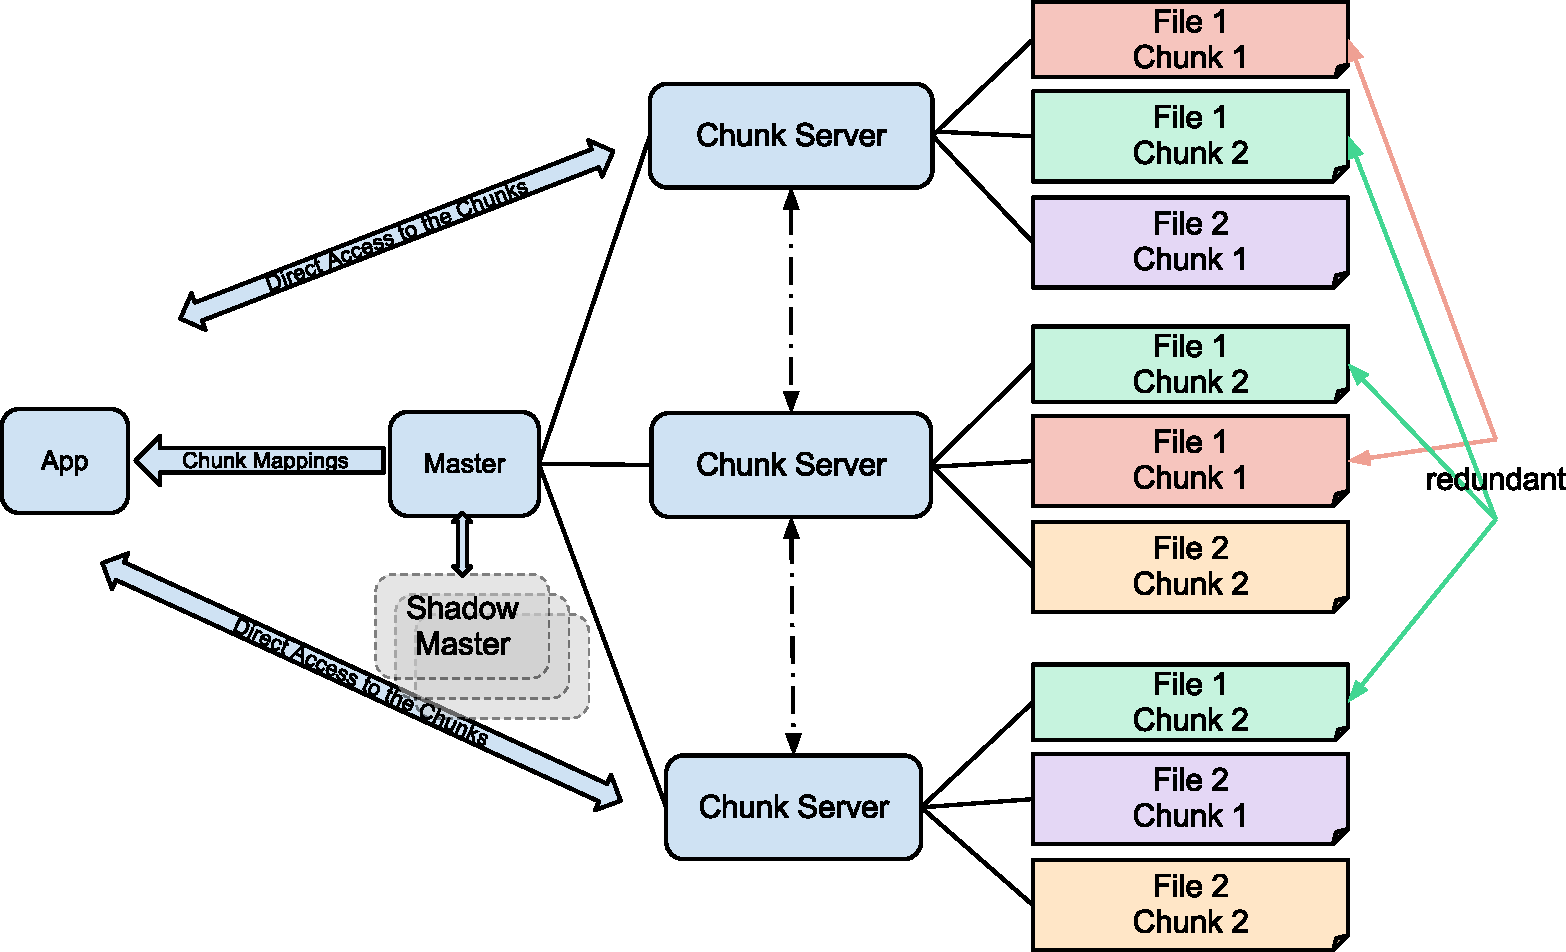
\includegraphics[width=\textwidth]{gfs-diagram.pdf}
    \caption{GFS architecture}
    \label{fig:architecture}
\end{figure}

On the server-side, there is a single \emph{master} controlling multiple slaves, known as \emph{chunkservers}. These are accessed by multiple clients, as shown in  Figure \ref{fig:architecture}.

The single master maintains all metadata. The metadata includes access control, mapping files to chunks, and mapping of chunks to the chunkservers which contain them.  The presence of a single master allows GFS to sidestep complex logic around multiple-sources-of-truth. 

Files are divided into fixed-size \emph{chunks}. Each chunk is identified by an immutable and globally unique 64 bit chunk handle assigned by the master at the time of chunk creation.  Chunkservers store chunks on local disks as Linux files and read or write chunk data specified by a chunk handle and offset. For reliability, each chunk gets replicated on multiple chunkservers. The user can modify the number of replicas stored; the default is 3. The master periodically communicates with each chunkserver in HeartBeat messages to give it instructions and collect its state.


Clients interact with the master for metadata operations, but all data-bearing communication goes directly to the chunkservers. This prevents bottlenecking the master; within GFS, lightweight control flow occurs by communication with the master; heavyweight dataflow is performed by directly talking to the chunk servers.

\subsubsection{Master Design}

We describe the design of the master in detail. In GFS, there is a \emph{single master} at any given moment. Being a single leader, the
master can take sophisticated chunk placement and replication decisions using global knowledge. The master is the central
point of communication through which all control flow occurs. Hence, any requests from the client
to read/write/modify must have the master as a signatory (control flow), before the client proceeds to perform the operation
with the chunkserver directly (data flow).

\subsubsection{Data Owned By Master}
The master stores three major types of metadata: the file and chunk namespaces, the mapping from files to chunks, and the locations of each chunk’s replicas.

All metadata is kept \textbf{in-memory}. The first two types (namespaces and file-to-chunkmapping) are also kept persistent by logging mutations to an operation log stored on the master’s local disk, and replicated on remote machines. Using a log allows us the master state to be updated simply, reliably, and without risking inconsistencies in the event of a master crash. 

The master does not store chunk location information persistently. Instead, it asks each chunkserver about its chunks at master startup and whenever a chunkserver joins the cluster.  Since metadata is stored in memory, master operations are fast. Furthermore, it is easy and efficient for the master to periodically scan through its entire state in the background. The master does not keep a persistent record of which chunkservers have a replica of a given chunk. It simply polls chunkservers for that information at startup. The master can keep itself up-to-date thereafter because it controls all chunk placement and monitors chunkserver status with regular HeartBeat message.

\paragraph{The Master Operation Log}
The operation log contains a historical record of critical metadata changes. It is a persistent record of metadata; it also serves as a logical time line  that defines the order of concurrent operations. 

Files, chunks, and their versions are all uniquely and eternally identified by the logical times at which they were created.  Since the operation log is critical, It must be stored reliably. Otherwise, one can  effectively lose the whole file system or recent client operations even if the chunks themselves survive, due to a loss of metadata of which chunk does what.  Therefore, the operation log is replicated on multiple remote machines; client operations are responded to only after flushing the corresponding log record to disk both locally and remotely.

The master recovers its file system state by replaying the operation log. To minimize startup time, the log is kept small through the use of checkpointing. The master checkpoints its state whenever the log grows beyond a certain size; this allows fast recovery by loading the latest checkpoint from local disk and replaying only the limited number of log records after that. A failure during checkpointing does not affect correctness because the recovery code detects and skips incomplete checkpoints.

\paragraph{Namespacing And Locking}
Many master operations can take a long time. We do not want to delay other master operations for one expensive operation. Therefore, we allow multiple
operations to be active and use locks over regions of the namespace to ensure
proper serialization.

Consider an example of how this locking mechanism can prevent a file \texttt{/home/user/foo} from being created while \texttt{/home/user} is being snapshotted to /save/user. The snapshot operation acquires read lock on  \texttt{/home} and \texttt{/save}, and write locks on \texttt{/home/user} and \texttt{/save/user}. The file creation acquires read locks on \texttt{/home} and \texttt{/home/user}, and a write lock
on \texttt{/home/user/foo}. The two operations will be serialized properly because they try to obtain conflicting locks on \texttt{/home/user}. 

File creation does not require a write lock on the parent directory because there is no 'directory'/ \texttt{inode} data structure to be protected from modification.  The read lock on the name is sufficient to protect the parent directory from deletion.

\subsection{Client operations}

\subsubsection{Reads}

The sequence of events for a client to fetch a file from GFS is:
\begin{itemize}
    \item[1]  The client wishes to read data from a file $f$ starting from byte offset $o$, of some length $l$. using the fixed chunk size, the client translates the byte offset into a chunk index ($b/\texttt{chunksize}$) within the file. It sends the request of (file, chunk index) to the master.
    \item[2]  The master replies with the corresponding chunk handle and locations of the replicas \emph{(control-flow)}.
    \item[3] The client caches this information using the file name and chunkindex as the key.
    \item[4] The client then sends a request to one of the replicas. The request specifies the chunk handle and a byte range within that chunk. \emph{(data-flow)}.
    \item[5] Further reads of the same chunk require no more client-master interaction.
\end{itemize}

\subsubsection{Mutations: Writes And Appends}

A mutation is an operation that changes the contents or metadata of a chunk such as a write or an append operation. Each mutation is performed at all the chunk’s replicas. Leases are used to maintain a consistent mutation order across replicas. The master grants a chunk lease to one of the replicas, which we call the \textbf{primary replica for that chunk}. The primary picks a serial order for all mutations to the chunk. All replicas follow this order when applying mutations. 

The lease mechanism is designed to minimize management overhead at the master. A lease has an initial timeout of 60 seconds. However, as long as the chunk is being mutated, the primary receive extensions from the master indefinitely. These extension requests and grants are piggybacked on the HeartBeat messages regularly exchanged between the master and all chunkservers.  The master may sometimes try to revoke a lease before it expires (e.g., when the master wants to disable mutations on a file that is being renamed). Even if the master loses communication with a primary, it can safely grant a new lease to another replica after the old lease expires.

The sequence of events from a client's perspective to perform a write are as follows:

\begin{itemize}
\item[1] The client asks the master which chunkserver holds the current lease for the chunk, and the locations of the other replicas. If no one has a lease, the master grants a lease to some replica.

\item[2] The master replies with the identity of the primary and the locations of the secondary replicas. The client caches this data for future mutations. The client contacts the master again only when the primary becomes unreachable or replies that it no longer holds a lease. 

\item[3] The client pushes the data to all the replicas. A client can do so in any order. This data is stored in a buffer in the replica; it is  \emph{not yet written}.

\item[4] Once all the replicas have acknowledged receiving the data, the client sends a write request to the primary. The request identifies the data pushed earlier to all of the replicas. The primary assigns consecutive serial numbers to all the mutations it receives, possibly from multiple clients, which provides the necessary serialization. It applies the mutation to its own local state in serial number order.

\item[5] The primary forwards the write request to all secondary replicas. Each secondary replica applies mutations in the same serial number order assigned by the primary.

\item[6] The secondaries all reply to the primary indicating that they have completed the operation.

\item[7] The primary replies to the client. Any errors encountered at any of the replicas are reported to the client.  In case of errors, the write may have succeeded at the primary and an arbitrary subset of the secondary replicas. (If it had failed at the primary, it would not have been assigned a serial number and forwarded.) The client request is considered to have failed, and the modified region is left in an inconsistent state. It is the responsibility of the client to handle such failures by retrying steps (3) through (7).
\end{itemize}

\subsection{Properties of GFS}

\subsubsection{Special support for \texttt{append}s}

Record append is heavily used to model many-producer-queues. 

In a traditional write, the client specifies the offset at which data is to b written. Concurrent writes to the same region are not serializable: the regio may end up containing data fragments from multiple clients. In a record append however, the client specifies only the data. GFS appends it to the file a least once atomically (i.e., as one continuous sequence of bytes) at an offs of GFS’s choosing and returns that offset to the client. 

If a record append fails at any replica, the client retries the operation. As  result, replicas of the same chunk may contain different data possibly including duplicates of the same record in whole or in part. GFS does not guarantee tha all replicas are bytewise identical. It only guarantees that the data is written at least once as an atomic unit. 

\subsubsection{Snapshot}

The snapshot operation makes a copy of a file or a directory tree (the “source”) almost instantaneously, while minimizing any interruptions of ongoing
mutations. This can be used to branch copies of huge data sets (and often copies of those copies, recursively), or to checkpoint the current state before experimenting with changes that can later be committed or rolled back. Copy-on-write is used to implement snapshots. 

When the master receives a snapshot request, it first revokes any outstanding leases on the chunks in the files it is about to snapshot. This ensures that any subsequent writes to these chunks will require an interaction with the master to find the lease holder. This will give the master an opportunity to create a new copy of the chunk first. 

After the leases have been revoked or have expired, the master logs the operation to disk. It then applies this log record to its in-memory state by duplicating the metadata for the source file or directory tree. The newly created snapshot files point to the same chunks as the source files.  The first time a client wants to write to a chunk \texttt{C} after the snapshot operation, it sends a request to the master to find the current lease holder. The master notices that the reference count for chunk \texttt{C} is greater than one. It defers replying to the client request and instead picks a new chunk handle \texttt{C’}.  It then asks each chunkserver that has a current replica of \texttt{C} to create a new chunk called \texttt{C’}. By creating the new chunk on the same chunkservers as the original, the data can be copied locally, not over the network.  From this point, request handling is no different from that for any chunk: the master grants one of the replicas a lease on the new chunk \texttt{C’} and replies to the client, which can write the chunk normally, not knowing that it has just been created from an existing chunk.

\section{MinIO}
Minio is an up-and-coming open-source cloud solution to distributed storage. Fighting with current proprietary solutions like that of Amazon, Google, and Facebook, Minio aims to enable application developers to create their own storage clouds.

Essentially an object store (even more simplistically, it could be considered an FTP server with get/put capabilities over http), the filesystem supports storage of objects up to a size of 5 TB, which is great for many usecases of storing unstructured data like: photos, videos, log files, backups and container images. 

Minio is built to be agnostic of the underlying hardware, and can easily be deployed in a large variety of virtualized and physical setups. It is specifically designed to be performant and easily can be used for peta-scale workloads. Additionally, this distributed filesystem offers many large-enterprise level features including: erasure coding, bitrot protection, encryption/WORM, identity management, continuous replication, global federation, and support for multi-cloud deployments via gateway mode.

Some of the feature highlights of Minio include:
\begin{itemize} 
    \item \textit{Hyperscale Architecture}: enabling multi-data center expansion through federation
    \item \textit{High Performance}: object store capable of serving demanding cloud-native workloads
    \item \textit{Ease of Use}: Easy to support, Non-disruptive upgrades, and no tuning knobs.
    \item \textit{High Availability}: so objects continue to be available despite multiple disk and node failures
    \item \textit{Security-Enabled Storage}: Each object is encrypted by a unique key.
\end{itemize}

\subsection{Goals of MinIO}
Philosophically, Minio is built to be minimal (thus the name). While best suited to store information "blobs", as an object store, it can handle almost all types of unstructured data. 

Minio aims to address some of the failings, especially of similar filesystems which support MapReduce type workloads, by identifying one of the core issues: the fact that storage and compute don't scale at the same rate. Following a client-server architecture, they allow separate scaling of compute and storage nodes, which helps with both high availability, and optimization of hardware.

Additionally, when dealing with big data on distributed setups, your data is almost always not sitting on the same system which your application is running on. With bigger worries like replication of storage and scaling storage, Minio provides an easy solution. By decoupling disk storage from the local machines themselves, and making them accessible through an http api, applications can be built without worrying about this data layer. On top of that, redundant data storage can easily be created without needing to deal with cluster filesystems, which add other overheads to the process.

By API design, Minio is meant to be a strong alternative to Amazon S3, which in some sense, is considered to be the gold standard with respect to back-end file storage for cloud applications. As a result, this can act as a free, local alternative to those businesses who don't want to trust their critical data sitting on other cloud providers. 

Simplistically, files are organised into logically separated “buckets” of data, and can be passed to your application along with your required authentication credentials along with the address of your minio instance.

\subsection{Architecture Description}
\begin{figure}
    \centering
    % \includegraphics[width=\linewidth]{MinIO.png}
    \caption{MinIO Architecture Diagram}
    \label{fig: minio}
\end{figure}

By design, MinIO is cloud native and can be run using lightweight containers managed by external orchestration services (ex. Kubernetes). A competitive advantage of Minio is that it fits the entire server into a single ~40MB static binary. Though not compiled at source, it is highly efficient in its use of CPU and memory resources and thus allows the co-hosting of a large number of tenants on shared hardware.

MinIO fucntions well on commodity servers (though often benchmarked with state-of-the-art hardware) with locally attached drives (JBOD/JBOF). Keeping to the norms of efficient scalability, all the servers in a cluster are equal in capability (fully symmetrical architecture). In fact, there are no name nodes or metadata servers.

An important implenentation detail within MinIO, is that it writes data and metadata together as objects thus eliminating the requirement for a separate metadata database. MinIO's resiliency can also be attributed to the fact that all functions it uses are inline and strictly consistent. 

While a MinIO cluster is a collection of distributed MinIO servers with one process per node, it itself runs in the user space as a single process and uses lightweight co-routines for high concurrency. A deterministic hashing algorithm is utilized to place objects within Erasure sets, which have 16 drives per set by default.

Architecturally MinIO is designed to operate at scale, across multi-datacenter cloud services. In it, each tenant runs their own fully-isolated MinIO cluster, protecting them from all possible disruptions to to things like upgrades, updates, and security breaches. Additionally, each tenant can scale independently by federating clusters across geographical locations. Minio's Object Storage Architecture is also quite interesting. Most existing storage solutions follow a system which involves a multi-layer storage architecture comprising a durable block layer at the bottom , filesystem as "middleware", and APIs on top implementing protocols for various operations on files, blocks and objects.

While public cloud architectures provide separate object, file and block storage, Minio follows a fundamentally different architecture: using a single layer to achieve everything. As a result, the minio object server is high-performance and lightweight. 

\subsubsection{MinIO Design Decisions}

\paragraph{Lambda* Function Support}
Enterprise standard messaging platforms can be used to deliver notifications of events via the Amazon-compatible lambda event notifications. This allows notifications for object level events / actions like: access, creation and deletion to be delivered to the application layer.


\paragraph{Linear Scaling}
By taking inspiration from hyperscalers, Minio clusters can be deployed at a wide range of nodes ranging from 4 to 32. Through its feature of Federation, multiple clusters are can easily be joined together under the same "global" namespace, which essentially is a single entity to the outside world. As a result of federation:
    \begin{itemize}
        \item All nodes are considered equal
        \item Any node can serve requests, concurrently
        \item A DLM (Distributed Locking Manager) helps a cluster manage updates and deletions
        \item There is no performance degradation of an individual cluster due to the addition of more clusters under the global namespace
        \item Cluster-level failure domain
    \end{itemize}

\paragraph{Erasure Code}
The integrity of object data is maintained by erasure coding and bitrot protection checksums. For some backgorund information, erasure code is a mathematical algorithm which can be used to reconstruct missing or corrupted data. To achieve this the Reed-Solomon code is used to shard objects into data and parity blocks, and hashing algorithms are used to help protect individual shards. As a result, Minio is resilient to silent data corruption (happens quite often at a peta-scale of data) and other hardware failures. Raid configurations and data replicas suffer from high storage overheads. Erasure code solves this problem while allowing for loss of up to 50 percent of drives and 50 percent of servers. RAID-6, as a case study, is only able to withstand two-drive failures. By applying erasure code to individual objects, Minio allows the healing of one object at a time. On the other hand, RAID-protected storage solutions have healing done at a RAID Volume level, which impacts performance for files within that level for the duration of the healing. 

\subsection{Properties of MinIO Distributed File System}
\begin{itemize}
    \item \textit{Performance}: One platform allows support for various different use cases. Industrial usecases have shown that a use rcan run  multiple Spark*, Presto* and Hive* queries, or even deploy large AI workloads and algorithms, without encountering any issues related to storage (read or write). Minio object storage allows for high throughput and low latency for cloud-native applications. Coupled with latest hardware and network infrastructure, Minio outperforms all traditional object storages. 
    \item \textit{Scalability}: Single clusters can be federated with other clusters to create namspaces which can span multiple datacenters. Incremental expansion of physical servers is what leads to the gradual expansion of the global namespace. Though a simple design, it leverages all cutting edge knowledge of hyperscalers. 
    \item \textit{Ease of Use}: Start up configuration time is only a few minutes, given the existence of a single 40MB binary for the server. Default configurations work very well, thus allowing for use in smaller projects as well, without full knowledge of system administration. 
    \item \textit{Encryption and WORM}: Unique keys are used to encrypt each object (per-object key). By supporting integration with external key management solutions, state of the art cryptography solutions can be used to secure and manage encryption keys, without having any coupling with Minio. WORM (write once, read many) mode prevents data tampering.
    \item \textit{Identity and Access Management}: Support for OpenID*-compatible identity management servers allows for secure and well-tested access control. Temporary rotating credentials within Minio prevent the need to embed long-term credentials within an application. 
    \item \textit{High Availability}: Even if a minio cluster loses up to 50\% of its drives and servers, Minio will continue to serve objects. Additionally, total rack failures are also mitigated (if the cluster is deployed across racks). These features are achieved by using Minio's distributed erasure code, which uses multiple redundant parity blocks to protect data. In case of datacenter level outages, there is also support for continuous mirroring to remote sites (disaster recovery). 
    \item \textit{Metadata Architecture}: As a result of not having a separate metadata store, all failures are contained to within an object and do not spillover to the rest of the system. Additionally, all operations within Minio are performed atomically at an object-level of granularity. Other data integrity requirements are satisfied by the existence of erasure code and bitrot hash per object. 
    \item \textit{Strict Consistency}: Strictly consistent operations allows for the system to survive crashed even in the middle of other workloads, without any loss to pre-existing data. This is highly useful in usecases related to machine-learning and other big data workloads.
    \item \textit{Geographic Namespace}: Using Minio's federation feature, users can opt to scale in an incremental fashion rather than having to deploy across data-centers via hyperscalers from the start itself. It can be deployed in units which have a failure domain restricted to the size at which it is currently scaled.
    \item \textit{Cloud-native design}: Kubernetes and other orchestration platforms can easily be used along with Minio's multi-instance and multi-tenant design. Containerized deployment of Minio leads to the use of these orchestration services for reliable scaling. Each instance of Minio is can be provisioned on demand, through self-service registration. While traditional monolithic storage systems (which has it's own disadvantages) do compete with Kubernetes resource management, they lack it's easily scalable nature and the ability to pack many tenants simultaneously on the same shared infrastructure.
    
\end{itemize}

\section{Comparing the DFSs}

\begin{table}[]
\centering
\caption{}
\label{tab:hdfsvsminio}
\begin{tabular}{|c|c|c|c|c|c|c|}
\hline
 \bf DFS &  \bf Written In &  \bf License & \bf Access API & \bf High Availability & \bf Shards & \bf Release \\
 \hline
 \it Minio & Go & Apache v2 & AWS S3 API  & Yes & Yes & 2014 \\
 \hline
 \it HDFS & Java & Apache v2 & Java and C client, HTTP  & Transparent master failover & No & 2005\\
 \hline
 \it GFS & \texttt{UNK} & Proprietary & Native File System API & Yes & Yes (by Spanner) & 2003 \\ 
 \hline
\end{tabular}
\end{table}

\subsection{HDFS vs MinIO}


While HDFS has been a long-standing player in the distributed filesystem market, Minio has shown been shown to outperform it many of its seminal tasks. Their core difference lies in the philosophy of storage. HDFS achieves its high throughput values by colocating compute and data on the same nodes. As a result they get to exploit fewer network calls and overcome the limitations of slow network access. However, as storage requirements tend to grow much faster than compute requirements, node scaling within HDFS tends to lead to wastage of compute resources.

An example of an issue caused by this would be that if HDFS were to have to store 10 petabytes of data, due to its replication factor of 3, it would need to store 30 petabytes on the whole. At a max storage of 100TB per node, this would need 300 nodes, which would clearly overprovision compute facilities, thus causing other overheads. 

Minio overcomes these issues by the natural solution of separating storage an compute resources. Along with it's cloud-native infrastructure, it is able to use orchestration frameworks like Kubernetes the software stack.

\subsubsection{Performance}
To compare performance of the two filesystems an experiment is set up. First the infrastructure is benchmarked, to see the baseline limitations of the setup.
\begin{itemize}
    \item Hard Drive Performance
        \begin{itemize}
            \item Write: 137 MB/s
            \item Read: 205 MB/s
            \item Multi-drive performance with 32 threads + 32kb blocks:
                \begin{itemize}
                    \item Write: 655 MB/s
                    \item Read: 1.26 GB/s
                \end{itemize}
        \end{itemize}
    \item Network Performance
        \begin{itemize}
            \item Ethernet cables support 3.125 GB/s, but with multiple connections the sustained throughput was at around 1.26 GB/s
        \end{itemize}
\end{itemize}

After the benchmarking of the basic infrastructure, some degree of tuning is done for each of the filesystems. This, on the whole, is to ensure that each of the filesystems are using all the resources allocated to them to the max extent possible, as would be done in a normal stress test.

\begin{itemize}
    \item Minio
        \begin{itemize}
            \item 1.2 TB aggregate memory across 12 nodes. Tuning done such that MapReduce jobs could use the whole allocated CPU and Memory provided by compute nodes.
            \item The entire 144GB of ram of each node was used.
            \item S3A connector (API) is tuned
        \end{itemize}
    \item HDFS
        \begin{itemize}
            \item Tuned to 2.4 TB aggregate memory across 12 nodes. 
            \item Tuned til the entirety of the 256 GB Ram on all compute nodes was being used. (Higher RAM due to shared compute and storage nodes).
            \item Ensured that computations do not go into swap space as well (as that causes lower performance)
            \item Configured to replicate data with a factor of 3
        \end{itemize}
\end{itemize}

The following tasks, which are considered to be Hadoop's most proven benchmarks, are evaluated:
\begin{itemize}
    \item Terasort
    \item Sort
    \item Wordcount
\end{itemize}


\subsection{HDFS vs GFS}
We use sources \cite{lecturehdfsvsgfs} and data published in the papers of HDFS
and GFS to draw comparisons.

GFS was built for the unique of Google as a company: The use of off-the-shelf
hardware to run production servers, their scale of batch data processing, the
generally append only nature of their high-throughput, latency-insensitive
workload. 

On the other hand, HDFS was implemented for the purpose of
running Hadoop’s MapReduce applications. It was created as an open-source
framework for the usage of different clients with different needs. This makes
Hadoop far less opinionated; Therefore, it is also far less optimized at handling
workloads that GFS is tuned for.

In terms of data storage, recall that GFS chunks data into 64 MB chunks that
are uniquely identified; These chunks are replicated into 64 KB blocks
which are checksummed. This permits fast chunked reads, while allowing
for error detection using the per-block checksum. On the other hand, HDFS 
divides data into  128MB blocks. The HDFS NameNode holds block replica
as two files: one with the data, the other with the checksum and generation stamp.

In terms of architecture, GFS is more involved, due to their focus on
concurrent, atomic appends and snapshotting support. In particular, GFS
require leases. The client is told where to write by the master. In HDFS,
the client decides where to write. 


We collate data about reads and writes from the data published by Google
on GFS performance as it runs on real-world clusters (Cluster B in )%\cite{ghemawat2003google}).
Similarly, for HDFS, we cite their busy read/write numbers from their runs
on the DFSIO test suite, with 3500 Nodes, using Hadoop MapReduce as a client
for HDFS.


\begin{table}[H]
\centering
\begin{tabular}{c c c}
\hline
 \bf Measurement &  \bf GFS &  \bf HDFS \\
 \hline
 \it Read (Busy)  & 380 MB/s &  1.02 MB/s/node \\
 \it Writes (Busy) & 117 MB/s  & 1.09 MB/s per node \\
 \end{tabular}
 \caption{performance comparison: HDFS v/s GFS on production workloads. HDFS data gathered using 3000 nodes on DFSIO
 test suite. GFS numbers from Google's reported performance in production}
\label{tab:hdfsvsgfs}
\end{table}

\section{Conclusion}

\nocite{*} % allow all bibs to show up, regardless of whether they have been cited.
\bibliographystyle{acm}
\bibliography{refs}
\end{document}
